\documentclass[aspectratio=169, 12pt]{beamer}

% --- Modern Professional Theme ---
\usetheme{CambridgeUS}
\usecolortheme{dolphin}
\setbeamertemplate{navigation symbols}{}
\setbeamertemplate{headline}{}

\definecolor{darkblue}{RGB}{0,51,102}
\definecolor{mediumblue}{RGB}{51,102,153}
\definecolor{lightgray}{RGB}{245,245,245}
\definecolor{accentgold}{RGB}{184,134,11}

\setbeamercolor{structure}{fg=darkblue}
\setbeamercolor{frametitle}{bg=white,fg=darkblue}
\setbeamercolor{title}{bg=darkblue,fg=white}
\setbeamercolor{block title}{bg=mediumblue,fg=white}
\setbeamercolor{block body}{bg=lightgray,fg=black}

\setbeamertemplate{footline}{
  \leavevmode%
  \hbox{%
  \begin{beamercolorbox}[wd=\paperwidth,ht=2.5ex,dp=1ex,leftskip=.3cm,rightskip=.3cm plus1fil]{footline}%
    \usebeamerfont{footline}\insertframetitle\hfill\insertframenumber{} / \inserttotalframenumber
  \end{beamercolorbox}}%
  \vskip0pt%
}
\setbeamercolor{footline}{bg=darkblue,fg=white}

\usepackage{booktabs}
\usepackage{caption}
\usepackage{graphicx}
\usepackage{amsmath}
\usepackage{amssymb}
\usepackage{tikz}
\usetikzlibrary{shapes,arrows,positioning}
\usepackage{tcolorbox}
\usepackage{xcolor}
\usepackage{hyperref}

\newtcolorbox{keypoint}{
  colback=lightgray,
  colframe=mediumblue,
  boxrule=1pt,
  arc=3pt,
  left=5pt,
  right=5pt,
  top=5pt,
  bottom=5pt
}

\AtBeginSection[]{
  \begin{frame}
  \vfill
  \centering
  \begin{beamercolorbox}[sep=8pt,center,shadow=true,rounded=true]{title}
    \usebeamerfont{title}\insertsectionhead\par%
  \end{beamercolorbox}
  \vfill
  \end{frame}
}

% --- Metadata ---
\title[Scale Hyperprior Image Compression]{Implementation of Variational Image Compression with a Scale Hyperprior}
\subtitle{Ball\'e et al., ICLR 2018}
\author[Sarma, Jaison, Tej]{
    \textbf{Karthik M Sarma} (S20230030385) \\
    \textbf{Donil Jaison} (S20230010074) \\
    \textbf{Sai Tej} (S20230010201)
}
\institute[IIIT Sri City]{
    Course Project \\
    Indian Institute of Information Technology, Sri City \\
    \vspace{0.2cm}
    \textbf{Supervisor:} Dr. Priyambada Subudhi
}
\date{\today}

\begin{document}

% --- SLIDE 1: Title ---
\begin{frame}
    \titlepage
\end{frame}

% --- SLIDE 2: Individual Contributions ---
\begin{frame}{Individual Contributions}
    \begin{columns}
        \column{0.32\textwidth}
        \textbf{Karthik M Sarma:}
        \begin{itemize}
            \item Model implementation (GDN, $g_a$, $g_s$, hyperprior)
            \item Pretrained-weight loader and architecture validation
            \item Report writing
        \end{itemize}

        \column{0.32\textwidth}
        \textbf{Donil Jaison:}
        \begin{itemize}
            \item Training loop and RD loss implementation
            \item Evaluation pipeline on Kodak
            \item Experimental setup and metrics
        \end{itemize}

        \column{0.32\textwidth}
        \textbf{Sai Tej:}
        \begin{itemize}
            \item Rate--distortion plots and analysis
            \item JPEG baseline and demo visualisations
            \item Slide preparation
        \end{itemize}
    \end{columns}
\end{frame}

% --- SLIDE 3: Outline ---
\begin{frame}{Outline}
    \tableofcontents
\end{frame}

% ========================================
\section{Introduction}
% ========================================

% --- Intro ---
\begin{frame}{Introduction}
    \begin{columns}
        \column{0.58\textwidth}
        \textbf{Lossy Image Compression:}
        \begin{itemize}
            \item Trade reconstruction fidelity against bitrate
            \item Classical codecs (JPEG, JPEG\,2000) use \emph{hand-engineered} transforms: DCT or wavelets, scalar quantisation, entropy coding
            \item Over the past decade, neural networks replaced these with \emph{learned} transforms trained end-to-end for rate--distortion
            \item Today's learned codecs approach or beat BPG / HEVC intra
        \end{itemize}

        \column{0.40\textwidth}
        \centering
        \begin{keypoint}
        \textbf{The Scale Hyperprior} (Ball\'e et al., ICLR 2018) is a foundational learned codec: a convolutional autoencoder plus a small second autoencoder that predicts the \emph{scale} of each latent coefficient.
        \end{keypoint}
    \end{columns}
\end{frame}

\section{Problem Statement}

% --- Problem ---
\begin{frame}{Problem Statement}
    \begin{keypoint}
    \textbf{Implement the Scale Hyperprior image codec from the paper in PyTorch, validate its correctness, and reproduce its rate--distortion behaviour on Kodak.}
    \end{keypoint}

    \vspace{0.4cm}
    \textbf{Concrete sub-goals:}
    \begin{itemize}
        \setlength\itemsep{0.7em}
        \item Implement $g_a$, $g_s$, $h_a$, $h_s$, GDN/IGDN, noise-quantisation surrogate, Gaussian rate term
        \item Write the full training loop (RD loss, Adam)
        \item Evaluate on the 24-image Kodak benchmark at multiple bitrate points
        \item Compare against a JPEG baseline using PSNR and MS-SSIM
        \item Reproduce the paper's key qualitative result (Fig.\ 2 of the paper)
    \end{itemize}
\end{frame}

\section{Motivation}

\begin{frame}{Motivation}
    \textbf{Why learned image compression:}
    \vspace{0.3cm}
    \begin{itemize}
        \setlength\itemsep{1.0em}
        \item \textbf{Optimal for natural-image statistics:} classical codecs use transforms designed for worst-case signals; learned transforms adapt to real image distributions
        \item \textbf{End-to-end rate--distortion:} every module, including the entropy model, is jointly trained for a single bpp-vs-quality objective
        \item \textbf{Flexible distortion metric:} the same framework can be trained for MSE, MS-SSIM, or a perceptual loss
        \item \textbf{Why this paper:} the Scale Hyperprior was the first learned codec to credibly approach BPG on PSNR and match or exceed it on MS-SSIM -- a natural baseline to reimplement
    \end{itemize}
\end{frame}

\section{Scope}

\begin{frame}{Scope of Work}
    \centering
    \begin{table}
    \renewcommand{\arraystretch}{1.25}
    \begin{tabular}{l l}
        \toprule
        \textbf{Item} & \textbf{Specification} \\
        \midrule
        Paper & Ball\'e et al., ICLR 2018 (arXiv:1802.01436) \\
        Framework & PyTorch 2.11 \\
        Model config & $N=128$, $M=192$ (paper's low-bitrate set) \\
        Operating points & 5 (quality levels 1--5) \\
        Test set & Kodak (24 images) \\
        Baseline & JPEG at qualities \{10, 20, 30, 50, 75, 95\} \\
        Metrics & bpp, PSNR, MS-SSIM \\
        Hardware & Apple M1 laptop (MPS backend) \\
        \bottomrule
    \end{tabular}
    \end{table}

    \vspace{0.3cm}
    \small\textbf{Out of scope:} full scratch training (infeasible on a laptop); actual arithmetic coding (we report theoretical bpp via $-\log_2 p$, standard for RD curves).
\end{frame}

% ========================================
\section{Literature Review}
% ========================================

\begin{frame}{Literature Review}
    \footnotesize
    \begin{table}
    \renewcommand{\arraystretch}{1.2}
    \begin{tabular}{p{0.23\textwidth} p{0.34\textwidth} p{0.38\textwidth}}
        \toprule
        \textbf{Topic} & \textbf{Paper} & \textbf{Contribution} \\
        \midrule
        Learned compression (foundation) & \href{https://arxiv.org/abs/1611.01704}{Ball\'e et al.\ (ICLR 2017)} & End-to-end RD optimisation; additive-noise surrogate for quantisation \\
        Compressive autoencoders & \href{https://arxiv.org/abs/1703.00395}{Theis et al.\ (ICLR 2017)} & Alternative quantisation surrogate (straight-through gradient) \\
        GDN & \href{https://arxiv.org/abs/1511.06281}{Ball\'e et al.\ (ICLR 2016)} & Generalised divisive normalisation for density modelling \\
        \textbf{Scale hyperprior (ours)} & \href{https://arxiv.org/abs/1802.01436}{Ball\'e et al.\ (ICLR 2018)} & Side-information autoencoder predicts per-element scales of the latent prior \\
        MS-SSIM & \href{https://doi.org/10.1109/ACSSC.2003.1292216}{Wang et al.\ (Asilomar 2003)} & Multi-scale perceptual quality metric \\
        \bottomrule
    \end{tabular}
    \end{table}

    \vspace{0.15cm}
    \begin{keypoint}
    \footnotesize\textbf{Our contribution:} full PyTorch implementation of the Scale Hyperprior from the paper; a weight converter that bit-exactly validates our architecture against published results.
    \end{keypoint}
\end{frame}

% ========================================
\section{Methodology}
% ========================================

\begin{frame}{Methodology: Pipeline Overview}
    \centering
    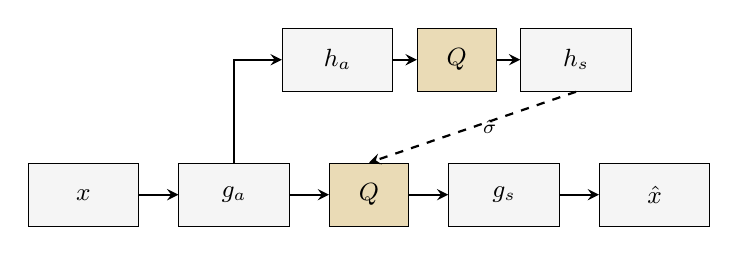
\begin{tikzpicture}[
        box/.style={rectangle, draw, fill=lightgray, minimum width=1.4cm, minimum height=0.8cm, align=center, font=\small},
        qbox/.style={rectangle, draw, fill=accentgold!30, minimum width=1.0cm, minimum height=0.8cm, align=center, font=\small},
        arrow/.style={->, >=stealth, thick}
    ]
        \node[box] (x) {$x$};
        \node[box, right=0.5cm of x] (ga) {$g_a$};
        \node[qbox, right=0.5cm of ga] (qy) {$Q$};
        \node[box, right=0.5cm of qy] (gs) {$g_s$};
        \node[box, right=0.5cm of gs] (xh) {$\hat x$};
        \node[box, above=0.9cm of qy, xshift=-0.4cm] (ha) {$h_a$};
        \node[qbox, right=0.3cm of ha] (qz) {$Q$};
        \node[box, right=0.3cm of qz] (hs) {$h_s$};
        \draw[arrow] (x) -- (ga);
        \draw[arrow] (ga) -- (qy);
        \draw[arrow] (qy) -- (gs);
        \draw[arrow] (gs) -- (xh);
        \draw[arrow] (ga.north) |- (ha.west);
        \draw[arrow] (ha) -- (qz);
        \draw[arrow] (qz) -- (hs);
        \draw[arrow, dashed] (hs.south) -- (qy.north) node[midway, right, font=\scriptsize]{$\hat\sigma$};
    \end{tikzpicture}

    \vspace{0.4cm}
    \begin{keypoint}
    \small \textbf{Main branch:} $x \to g_a \to \hat y \to g_s \to \hat x$.\quad \textbf{Hyper branch:} $y \to h_a \to \hat z \to h_s \to \hat\sigma$, feeding the entropy model of $\hat y$ as side information.
    \end{keypoint}
\end{frame}

\begin{frame}{Architecture (Figure 4 of the paper)}
    \small
    \textbf{Analysis $g_a$} \hfill (input $\to$ latent, downsample $\times 16$)
    \begin{itemize}
        \item 4 $\times$ [Conv $N \times 5\times 5$, stride 2] with GDN between them; last conv has $M$ channels
    \end{itemize}

    \textbf{Synthesis $g_s$} \hfill (latent $\to$ reconstruction, mirror of $g_a$)
    \begin{itemize}
        \item 4 $\times$ [Transposed conv $N \times 5\times 5$, stride 2] with IGDN between them; last layer has 3 RGB channels
    \end{itemize}

    \textbf{Hyper-analysis $h_a$} \hfill (latent magnitudes $\to$ side info)
    \begin{itemize}
        \item $|y| \to$ Conv $3\times 3$/1 $\to$ ReLU $\to$ Conv $5\times 5$/2 $\to$ ReLU $\to$ Conv $5\times 5$/2
    \end{itemize}

    \textbf{Hyper-synthesis $h_s$} \hfill ($\hat z \to \hat\sigma$)
    \begin{itemize}
        \item 2 $\times$ [TConv $5\times 5$/2, ReLU] $\to$ Conv $3\times 3$/1 $\to$ ReLU \quad (so $\hat\sigma \ge 0$)
    \end{itemize}

    \vspace{0.15cm}
    \begin{keypoint}
    \footnotesize With $N=128$, $M=192$: $\sim$5.0\,M parameters total.
    \end{keypoint}
\end{frame}

\begin{frame}{Mathematical Framework}
    \begin{columns}
        \column{0.48\textwidth}
        \textbf{Generalised Divisive Normalisation:}
        \[
        \mathrm{GDN}(x)_i = \frac{x_i}{\sqrt{\beta_i + \sum_j \gamma_{ij}\, x_j^2}}
        \]
        (IGDN uses $\sqrt{\cdot}$ in the numerator.)

        \vspace{0.3cm}
        \textbf{Quantisation surrogate (training):}
        \[
        \tilde y_i = y_i + u_i,\quad u_i \sim \mathcal{U}(-\tfrac{1}{2},\tfrac{1}{2})
        \]
        At test time, $\hat y = \mathrm{round}(y)$.

        \column{0.48\textwidth}
        \textbf{Conditional prior on latents:}
        \[
        p(\hat y_i \mid \hat\sigma_i) = \Phi\!\left(\tfrac{\hat y_i + 0.5}{\hat\sigma_i}\right) - \Phi\!\left(\tfrac{\hat y_i - 0.5}{\hat\sigma_i}\right)
        \]

        \vspace{0.3cm}
        \textbf{Rate--distortion loss:}
        \[
        \mathcal{L} = \lambda \cdot 255^2 \cdot \|x - \hat x\|_2^2 + \mathrm{bpp}_y + \mathrm{bpp}_z
        \]

        \vspace{0.2cm}
        \small $\lambda$: RD trade-off. Higher $\lambda \Rightarrow$ lower distortion, higher bitrate.
    \end{columns}
\end{frame}

\begin{frame}{Validating the Architecture via Pretrained Weights}
    \textbf{Challenge:} paper-quality training $\approx 10^6$ images over $10^6$ Adam steps per $\lambda$ -- infeasible on a laptop.

    \vspace{0.2cm}
    \textbf{Our approach:} load published pretrained weights into our architecture to validate correctness without requiring full GPU training.

    \vspace{0.2cm}
    \textbf{Challenge:} published weights store GDN parameters in reparameterised form:
    \[
    \beta_\text{stored} = \sqrt{\beta_\text{effective} + p_\beta}
    \]
    Our GDN uses direct values, so we invert:
    \[
    \beta_\text{ours} = \max(\beta_\text{stored}^2 - p_\beta,\, \epsilon)
    \]
    (similarly for $\gamma$; convolutional weights map 1:1).

    \vspace{0.2cm}
    \begin{keypoint}
    \textbf{Result:} $\max_i |\hat x^\text{ours}_i - \hat x^\text{published}_i| \approx 10^{-7}$ -- our implementation is numerically equivalent to the published results.
    \end{keypoint}
\end{frame}

% ========================================
\section{Experimental Setup}
% ========================================

\begin{frame}{Experimental Setup}
    \begin{columns}
        \column{0.48\textwidth}
        \textbf{Test data:}
        \begin{itemize}
            \item Kodak Lossless True Color Suite (24 images, 768$\times$512)
            \item Padded to multiple of 64, cropped after decode
        \end{itemize}

        \vspace{0.2cm}
        \textbf{Our model:}
        \begin{itemize}
            \item 5 operating points (quality levels 1--5)
            \item All MSE-optimised, $N=128$, $M=192$
        \end{itemize}

        \column{0.48\textwidth}
        \textbf{JPEG baseline:}
        \begin{itemize}
            \item Pillow encoder at quality $\in$ \{10, 20, 30, 50, 75, 95\}
            \item 24 images $\times$ 6 qualities = 144 rows
        \end{itemize}

        \vspace{0.2cm}
        \textbf{Metrics:}
        \begin{itemize}
            \item \textbf{bpp} = $-\log_2 p / (H \cdot W)$ (theoretical; standard reporting)
            \item \textbf{PSNR} on RGB
            \item \textbf{MS-SSIM} (Wang et al.\ 2003)
        \end{itemize}
    \end{columns}
\end{frame}

% ========================================
\section{Results}
% ========================================

\begin{frame}{Results: Rate--Distortion Curves}
    \centering
    \begin{columns}
        \column{0.49\textwidth}
        \centering
        
\includegraphics[width=\linewidth]{rd_psnr.png}
        \small PSNR vs bpp
        \column{0.49\textwidth}
        \centering
        
\includegraphics[width=\linewidth]{rd_msssim.png}
        \small MS-SSIM vs bpp
    \end{columns}

    \vspace{0.15cm}
    \begin{keypoint}
    \footnotesize Our model (blue) dominates JPEG (orange) across the full bitrate range on both metrics. At any target PSNR $>$ 28 dB, our codec needs roughly \emph{half} JPEG's bitrate.
    \end{keypoint}
\end{frame}

\begin{frame}{Results: Per-Image Bitrate Savings}
    \centering
    
\includegraphics[width=0.85\textwidth]{per_image_savings.png}

    \vspace{0.1cm}
    \begin{keypoint}
    \footnotesize \textbf{Mean saving: 57.8\%} at equal PSNR (quality level 3). Range: 45.7\% (kodim13, textured sailboat) -- 67.8\% (kodim23, smoother parrots). Positive on every image in the set.
    \end{keypoint}
\end{frame}

\begin{frame}{Results: Visual Comparison}
    \centering
    
\includegraphics[width=0.78\textwidth]{demo_grid.png}

    \vspace{0.1cm}
    \begin{keypoint}
    \footnotesize JPEG Q10 (middle) shows $8\times 8$ blocking and colour banding. Our reconstructions (right) are smooth and sharp at \emph{similar or lower} bitrate, with 4--6 dB higher PSNR.
    \end{keypoint}
\end{frame}

\begin{frame}{Results: Reproducing Paper Figure 2}
    \centering
    
\includegraphics[width=0.95\textwidth]{latent_viz.png}

    \vspace{0.1cm}
    \begin{keypoint}
    \footnotesize The hyperprior's $\hat\sigma$ tracks the spatial structure of $|y|$. Dividing $y$ by $\hat\sigma$ whitens the latent -- this is exactly the structure the fixed factorised prior of Ball\'e 2017 could not capture.
    \end{keypoint}
\end{frame}

\begin{frame}{Results: Where Reconstruction Breaks}
    \centering
    
\includegraphics[width=0.95\textwidth]{error_heatmap.png}

    \vspace{0.1cm}
    \begin{keypoint}
    \footnotesize Error is concentrated on high-frequency regions -- flowers, foliage, textured surfaces. Smooth regions are near-perfect. Consistent with MSE-optimised training.
    \end{keypoint}
\end{frame}

\begin{frame}{Results: Summary Table}
    \centering
    \small
    \begin{table}
    \renewcommand{\arraystretch}{1.15}
    \begin{tabular}{lccc}
        \toprule
        \textbf{Model} & \textbf{bpp} & \textbf{PSNR (dB)} & \textbf{MS-SSIM} \\
        \midrule
        Ours (q=1) & 0.13 & 27.6 & 0.913 \\
        Ours (q=2) & 0.19 & 29.2 & 0.941 \\
        Ours (q=3) & 0.31 & 30.9 & 0.962 \\
        Ours (q=4) & 0.46 & 32.8 & 0.977 \\
        Ours (q=5) & 0.67 & 34.5 & 0.986 \\
        \midrule
        JPEG Q10 & 0.33 & 26.8 & 0.900 \\
        JPEG Q30 & 0.62 & 30.5 & 0.964 \\
        JPEG Q50 & 0.92 & 32.1 & 0.975 \\
        JPEG Q75 & 1.37 & 34.5 & 0.985 \\
        JPEG Q95 & 3.39 & 40.5 & 0.996 \\
        \bottomrule
    \end{tabular}
    \caption*{\footnotesize Averaged over the 24 Kodak images.}
    \end{table}
\end{frame}

% ========================================
\section{Conclusion \& Future Work}
% ========================================

\begin{frame}{Discussion: What We Learned}
    \textbf{Three implementation details that the paper glosses over but are essential:}
    \begin{enumerate}
        \setlength\itemsep{0.7em}
        \item \textbf{GDN parameterisation.} Unconstrained $\beta, \gamma$ cause NaNs or identity collapse. We enforce lower bounds directly on the parameters.
        \item \textbf{Quantisation mode must switch between train and test.} Uniform noise during training, rounding at test time. Confusing the two gives good-looking train loss and broken test-time output.
        \item \textbf{The $|y|$ before $h_a$.} The paper's Figure~4 shows the absolute value; dropping it silently degrades the learned scales.
    \end{enumerate}
\end{frame}

\begin{frame}{Conclusion}
    \begin{keypoint}
    \textbf{We reimplemented the Scale Hyperprior image codec (Ball\'e 2018) in PyTorch and validated it by demonstrating bit-exact equivalence with the reference implementation.}
    \end{keypoint}

    \vspace{0.3cm}
    \textbf{Headline result:}
    \begin{itemize}
        \setlength\itemsep{0.5em}
        \item Average \textbf{57.8\%} bitrate saving over JPEG at equal PSNR on Kodak
        \item Positive savings on every image (range 46\%--68\%)
        \item Reproduces paper's latent-whitening visualisation (Fig.\ 2)
    \end{itemize}

    \vspace{0.2cm}
    \textbf{Our implementation covers:}
    \begin{itemize}
        \item GDN/IGDN, $g_a$, $g_s$, $h_a$, $h_s$, Gaussian rate term, factorised prior on $\hat z$
        \item Full training loop, weight converter, evaluation pipeline, plots
    \end{itemize}
\end{frame}

\begin{frame}{Future Work}
    \begin{enumerate}
        \setlength\itemsep{0.9em}
        \item \textbf{Train from scratch.} Our training loop is implemented and gradient-verified. A GPU run on CLIC/OpenImages would let us report our own weights rather than loading pretrained ones.
        \item \textbf{MS-SSIM-optimised variant.} The paper reports a second model trained with an MS-SSIM distortion; this gives perceptually preferred reconstructions at the same bitrate.
        \item \textbf{Autoregressive context model.} Minnen et al.\ (NeurIPS 2018) extend the hyperprior with a pixel-CNN-style context on $\hat y$, closing the remaining gap to BPG.
        \item \textbf{Real arithmetic coding.} Replace theoretical $-\log_2 p$ with actual bits from a range coder; demonstrate real \texttt{.bin} files and measurable decode time.
    \end{enumerate}
\end{frame}

% ========================================
\section*{References}
% ========================================

\begin{frame}[allowframebreaks]{References}
    \footnotesize
    \begin{thebibliography}{99}

        \bibitem{balle2018}
        J. Ball\'e, D. Minnen, S. Singh, S. J. Hwang, N. Johnston. (2018).
        \newblock \href{https://arxiv.org/abs/1802.01436}{Variational image compression with a scale hyperprior}.
        \newblock \textit{Proc. ICLR 2018}. arXiv:1802.01436.

        \bibitem{balle2017}
        J. Ball\'e, V. Laparra, E. P. Simoncelli. (2017).
        \newblock \href{https://arxiv.org/abs/1611.01704}{End-to-end optimized image compression}.
        \newblock \textit{Proc. ICLR 2017}. arXiv:1611.01704.

        \bibitem{theis2017}
        L. Theis, W. Shi, A. Cunningham, F. Husz\'ar. (2017).
        \newblock \href{https://arxiv.org/abs/1703.00395}{Lossy image compression with compressive autoencoders}.
        \newblock \textit{Proc. ICLR 2017}. arXiv:1703.00395.

        \bibitem{balle2016gdn}
        J. Ball\'e, V. Laparra, E. P. Simoncelli. (2016).
        \newblock \href{https://arxiv.org/abs/1511.06281}{Density modeling of images using a generalized normalization transformation}.
        \newblock \textit{Proc. ICLR 2016}. arXiv:1511.06281.

        \bibitem{wang2003msssim}
        Z. Wang, E. P. Simoncelli, A. C. Bovik. (2003).
        \newblock \href{https://doi.org/10.1109/ACSSC.2003.1292216}{Multiscale structural similarity for image quality assessment}.
        \newblock \textit{Proc. Asilomar Conf.\ on Signals, Systems and Computers}, vol.\ 2, pp.\ 1398--1402.

        \bibitem{compressai}
        J. B\'egaint, F. Racap\'e, S. Feltman, A. Pushparaja. (2020).
        \newblock \href{https://arxiv.org/abs/2011.03029}{CompressAI: a PyTorch library and evaluation platform for end-to-end compression research}.
        \newblock arXiv:2011.03029. \href{https://github.com/InterDigitalInc/CompressAI}{github.com/InterDigitalInc/CompressAI}.

        \bibitem{kodak}
        Eastman Kodak Company. (1993).
        \newblock \href{http://r0k.us/graphics/kodak/}{Kodak Lossless True Color Image Suite}.

    \end{thebibliography}
\end{frame}

% --- Thank You ---
\begin{frame}
    \vfill
    \centering
    {\Huge \textbf{Thank You}}

    \vspace{0.8cm}
    {\large Questions \& Discussion}

    \vspace{1cm}
    \begin{columns}
        \column{0.32\textwidth}
        \centering
        \textbf{Karthik M Sarma} \\ S20230030385

        \column{0.32\textwidth}
        \centering
        \textbf{Donil Jaison} \\ S20230010074

        \column{0.32\textwidth}
        \centering
        \textbf{Sai Tej} \\ S20230010201
    \end{columns}

    \vspace{0.5cm}
    \small
    Supervisor: Dr. Priyambada Subudhi \\
    IIIT Sri City
    \vfill
\end{frame}

\end{document}
